\documentclass[aspectratio=169]{beamer}
\usepackage[T1]{fontenc}
\usepackage{multicol}
\usepackage{ragged2e}   %new code
\usepackage[utf8]{inputenc}
\usepackage[brazil]{varioref, babel}
\usepackage[square,sort,comma,super]{natbib}
\usepackage{xmpmulti}
\usepackage{epsfig}
\usepackage{subcaption}
\usepackage{siunitx}
\usepackage{mathtools}
\usepackage{amssymb}
\usepackage{amsmath}
\usepackage{booktabs}
\usepackage{pbox}
\usepackage{graphicx,url}
\usepackage{etoolbox}
\usepackage{ru,hyperref,url} % 
\graphicspath{{../figures/}}

\usepackage{tikz}
\usetikzlibrary{shapes,arrows,fit, positioning, arrows.meta}
\usetikzlibrary{backgrounds}
\usepgflibrary{shapes.multipart}

\addtobeamertemplate{block begin}{}{\justifying}
\setbeamertemplate{section in toc}[sections numbered]

% The title of the presentation:
%  - first a short version which is visible at the bottom of each slide;
%  - second the full title shown on the title slide;

\title[XXIX Congresso de Iniciação Científica - UNICAMP]{
 Predição de Séries Temporais Baseada em Redes Neurais
Artificiais}

% Optional: a subtitle to be dispalyed on the title slide
% \subtitle{Show where you're from}

% The author(s) of the presentation:
%  - again first a short version to be displayed at the bottom;
%  - next the full list of authors, which may include contact information;
\author[João Pedro O. Pagnan]{ \footnotesize
  Aluno: João Pedro de Oliveira Pagnan [FEEC/UNICAMP]\\
  Orientador: Prof. Dr. Levy Boccato [FEEC/UNICAMP]\\
  Coorientador: Prof. Dr. Romis Ribeiro de Faissol Attux [FEEC/UNICAMP]\\\medskip
  }

% The institute:
%  - to start the name of the university as displayed on the top of each slide
%    this can be adjusted such that you can also create a Dutch version
%  - next the institute information as displayed on the title slide
\institute[Universidade Estadual de Campinas ]{
  Departamento de Engenharia de Computação e Automação Industrial -- DCA \\
  }

% Add a date and possibly the name of the event to the slides
%  - again first a short version to be shown at the bottom of each slide
%  - second the full date and event name for the title slide
\date{\scriptsize \today}

\begin{document}

\begin{frame}
  \titlepage
\end{frame}

\begin{frame}{Seções}
\begin{multicols}{2}
    \footnotesize \tableofcontents
\end{multicols}
\end{frame}

% Section titles are shown in at the top of the slides with the current section 
% highlighted. Note that the number of sections determines the size of the top 
% bar, and hence the university name and logo. If you do not add any sections 
% they will not be visible.
\section{Introdução}
\subsection{Previsão de séries temporais de sistemas caóticos}
\begin{frame}
    \frametitle{Introdução}
    \framesubtitle{Previsão de séries temporais de sistemas caóticos}
    \justifying A predição de séries temporais é uma das aplicações mais interessantes do tratamento de informação. O desafio de antecipar padrões de comportamento e construir modelos que sejam apropriados para explicar determinados fenômenos da natureza tem importância para a:
    
    \begin{itemize}[<+-| alert@+>]
        \item Biologia,
        \item Economia,
        \item Automação Industrial,
        \item Meteorologia,
        \item e várias outras áreas da ciência.
    \end{itemize}
\end{frame}

\begin{frame}
    \frametitle{Introdução}
    \framesubtitle{Previsão de séries temporais de sistemas caóticos}
    \justifying Uma classe de sistemas dinâmicos particularmente relevante dentro do contexto de modelagem e predição de séries temporais está ligada à ideia de dinâmica caótica. Apesar de serem determinísticos, esses sistemas são extremamente sensíveis às condições iniciais \cite{fiedler1994caos}.

\end{frame}

\begin{frame}
    \frametitle{Introdução}
    \framesubtitle{Previsão de séries temporais de sistemas caóticos}
    \justifying Tal característica intensifica o desafio de predizer as séries temporais originadas por eles, pois uma pequena incerteza na medida afetará toda a previsão. 

\end{frame}

\subsection{Previsão de séries temporais com redes neurais artificiais}

\begin{frame}
    \frametitle{Introdução}
    \framesubtitle{Previsão de séries temporais com redes neurais artificiais}
    \justifying Tendo em vista o desempenho de modelos não-lineares para previsão de diversas séries temporais \cite{connor1994recurrent}, optamos por estudar a aplicabilidade de redes neurais artificiais à previsão de séries relacionadas a sistemas com dinâmica caótica. 
    
    Esta pesquisa comparou o desempenho de quatro arquiteturas de redes neurais artificiais:
    
    \begin{itemize}[<+-| alert@+>]
	\item \textit{Multilayer Perceptron} (MLP) \cite{rosenblatt1958perceptron},
	\item \textit{Long Short-Term Memory} (LSTM) \cite{connor1994recurrent},
	\item \textit{Gated Recurrent Unit} (GRU) \cite{cho2014learning},
	\item \textit{Echo State Network} (ESN) \cite{jaeger2007echo}.
    \end{itemize} 
\end{frame}

\section{Cenários escolhidos}

\begin{frame}
    \frametitle{Cenários escolhidos}
    \justifying A comparação foi realizada considerando quatro cenários, sendo dois destes a tempo discreto e dois a tempo contínuo, sendo que foi gerado um conjunto de $5000$ amostras para cada sistema analisado. Os cenários escolhidos foram as séries temporais dos sistemas caóticos:

    \begin{itemize}[<+-| alert@+>]    
    \item Mapa de Hénon \cite{henon1976two},
    \item Mapa logístico \cite{may1976simple},
    \item Sistema de Lorenz \cite{lorenz1963deterministic},
    \item Equações de Mackey-Glass \cite{mackey1977oscillation}.
    \end{itemize}
\end{frame}

\subsection{Mapa de Hénon}
\begin{frame}
	\frametitle{Cenários escolhidos}
	\framesubtitle{Mapa de Hénon}
	\justifying Esse sistema foi proposto por Michel Hénon em 1976 como um modelo simplificado de uma seção de Poincaré do atrator de Lorenz, sendo descrito pelas equações abaixo \cite{henon1976two}:
\begin{subequations}
\begin{equation}
x[n+1] = y[n] + 1 - a\cdot (x[n])^2
\end{equation}
\begin{equation}
y[n+1] = b \cdot x[n]
\end{equation}
\end{subequations}
\end{frame}

\begin{frame}
	\frametitle{Cenários escolhidos}
	\framesubtitle{Mapa de Hénon}
\justifying Para esta pesquisa, foram utilizados os valores usuais para os parâmetros $a$ e $b$. Logo, têm-se que $a = 1.4$ e $b = 0.3$. Além disso, neste e nos outros sistemas. A figura \ref{fig:henon} mostra a série temporal referente à variável $x$ e o atrator obtido com a simulação para $[x[0]\; y[0]]^T = [1\; 0]^T$.
\begin{figure}[H]
     \begin{subfigure}[t]{0.3\textwidth}
         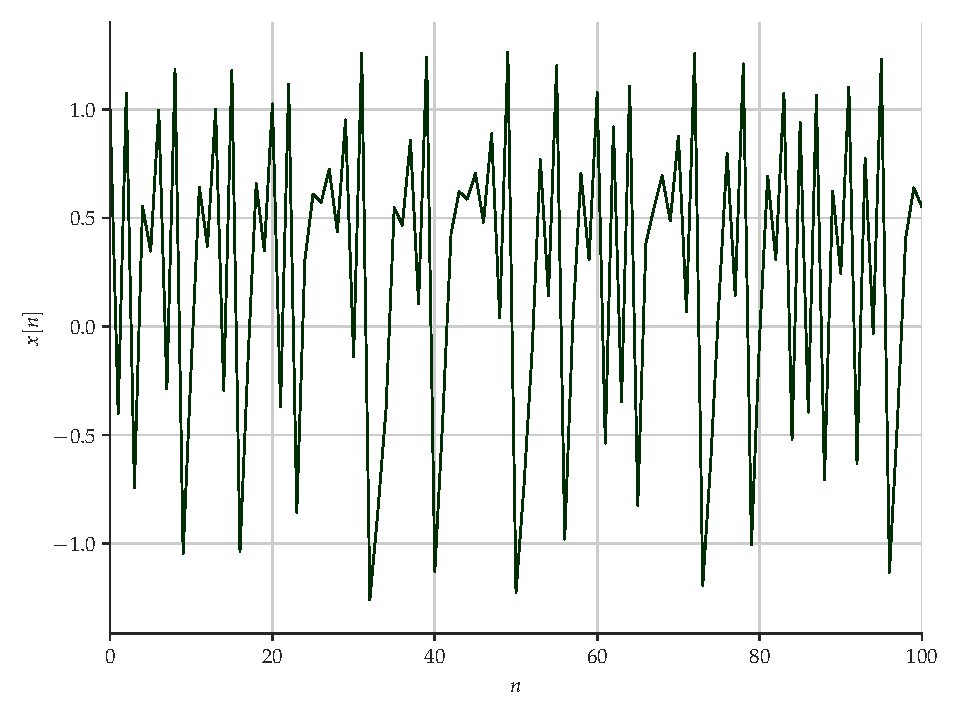
\includegraphics[scale=0.2]{serie-henon-x.pdf}
     \end{subfigure}
     \centering
     \begin{subfigure}[t]{0.3\textwidth}
         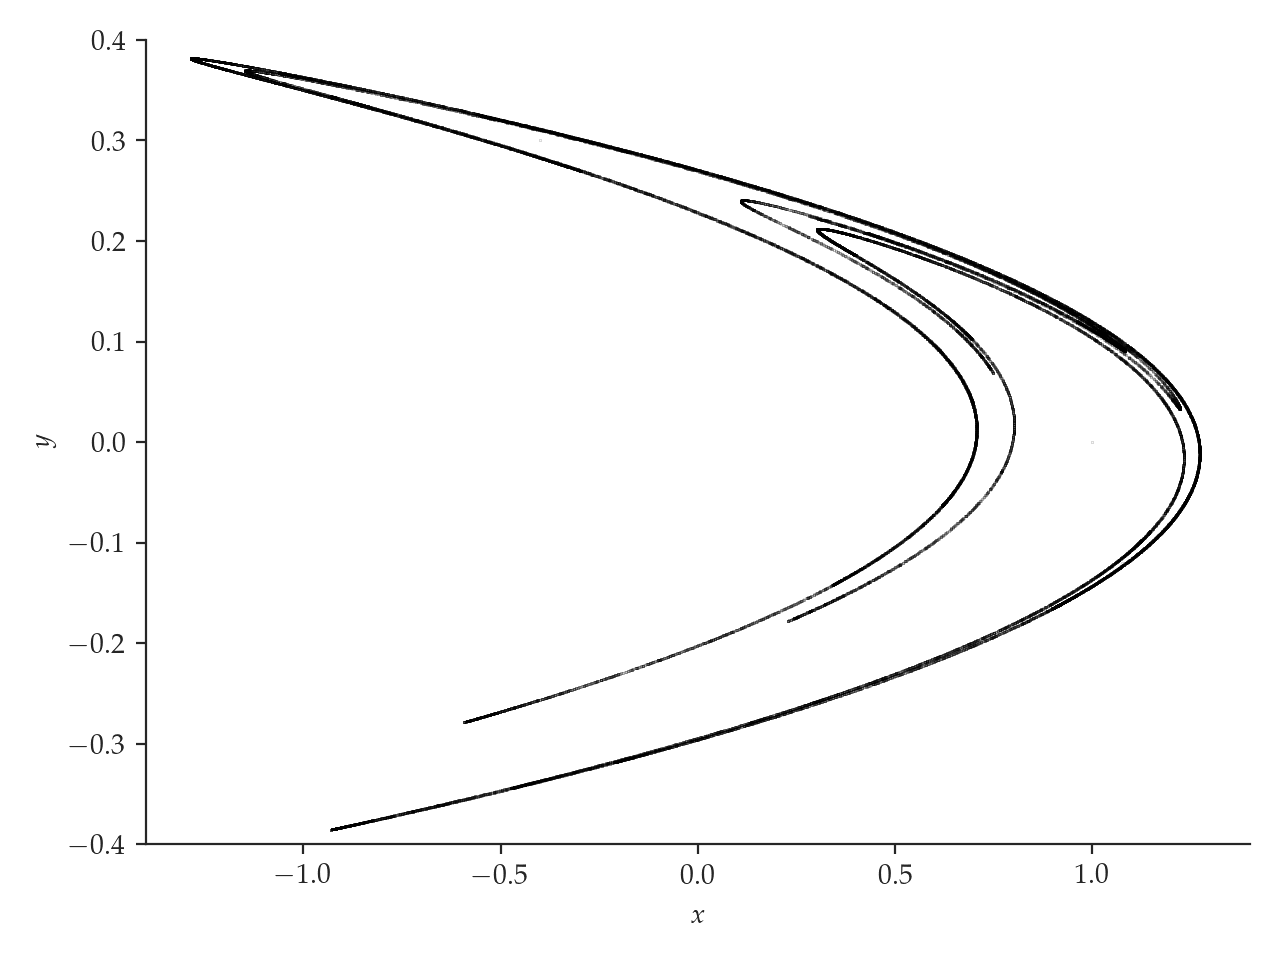
\includegraphics[scale=0.2]{mapa-de-henon.png}
     \end{subfigure}
     \caption{À esquerda, as cem primeiras iterações da série temporal em $x$ do mapa de Hénon e, à direita, o atrator correspondente à simulação}
     \label{fig:henon}
\end{figure}
\end{frame}

\subsection{Mapa logístico}
\begin{frame}
	\frametitle{Cenários escolhidos}
	\framesubtitle{Mapa logístico}
	\justifying Descrito em 1976 por Robert May, o mapa logístico representa uma das formas de modelar a população de uma determinada espécie em certos instantes de tempo \cite{may1976simple}. A equação a diferenças que descreve este sistema pode ser vista abaixo:
\begin{equation}\label{eq:logistic}
x[n+1] = r\cdot x[n] \cdot (1 - x[n])
\end{equation}
\end{frame}

\begin{frame}
	\frametitle{Cenários escolhidos}
	\framesubtitle{Mapa logístico}
\justifying Como o estudo visa analisar o desempenho para sistemas caóticos, foi utilizado $r=3.86$, que, conforme será visto no diagrama de bifurcação abaixo, faz com que a série temporal dada pela equação (\ref{eq:logistic}) opere em caos.
\begin{figure}[H]
     \begin{subfigure}[t]{0.3\textwidth} 
         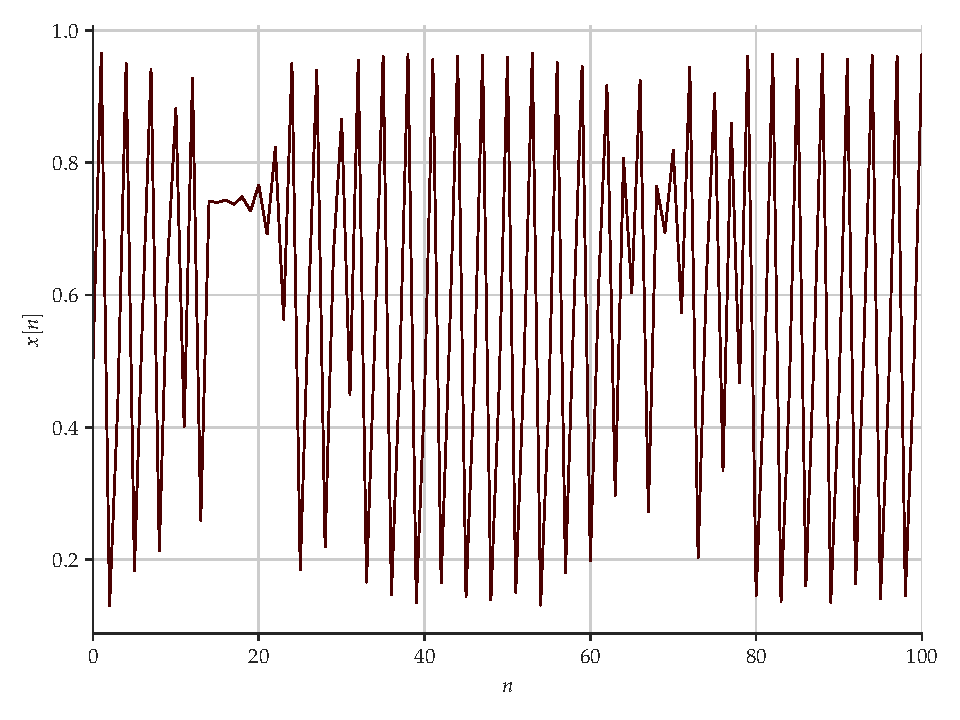
\includegraphics[scale=0.2]{serie-logistico.pdf}
         %\caption{$y=5/x$}
     \end{subfigure}
     \centering
     \begin{subfigure}[t]{0.3\textwidth} 
         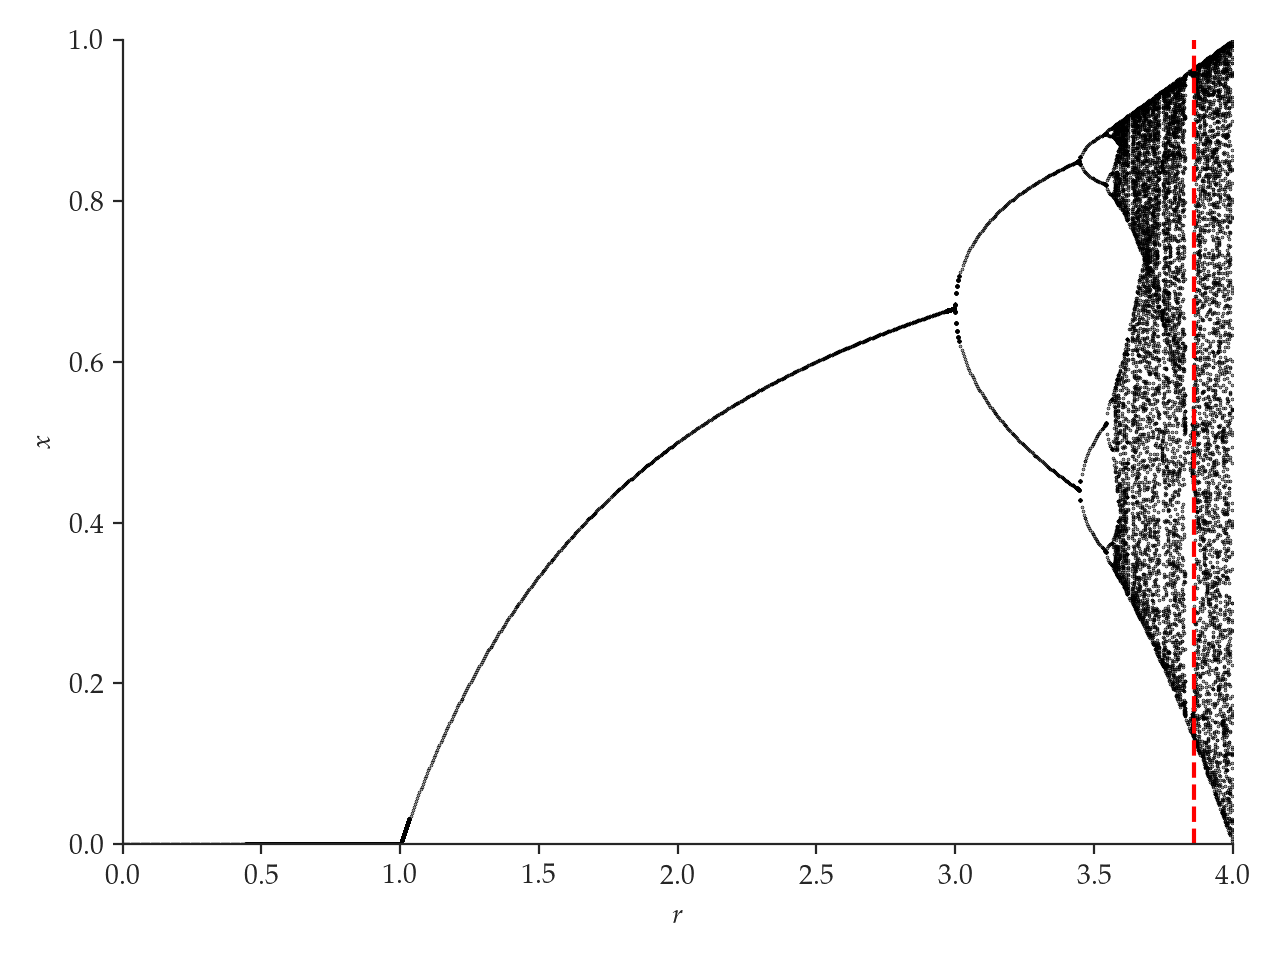
\includegraphics[scale=0.2]{mapa-logistico.png}
         %\caption{$y=x$}
     \end{subfigure}
     \begin{subfigure}[t]{0.3\textwidth} 
         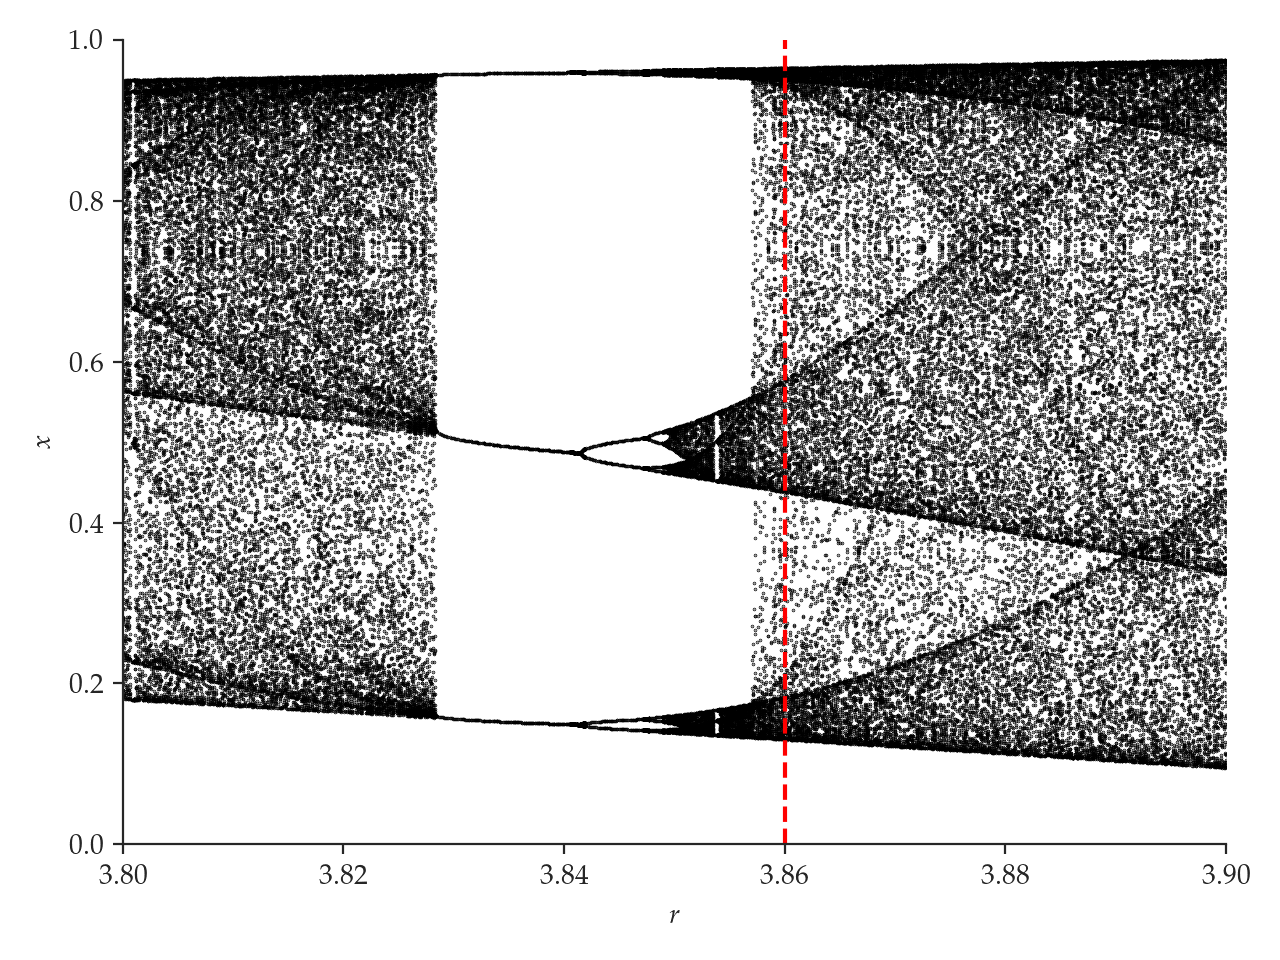
\includegraphics[scale=0.2]{mapa-logistico-zoom.png}
         %\caption{$y=x$}
     \end{subfigure}     
     \caption{À esquerda, as cem primeiras iterações da série temporal do mapa logístico e, à direita, o diagrama de bifurcação deste sistema}
     \label{fig:logistic}
\end{figure}
\end{frame}

\subsection{Sistema de Lorenz}

\begin{frame}
	\frametitle{Cenários escolhidos}
	\framesubtitle{Sistema de Lorenz}
\justifying Num dos primeiros grandes trabalhos envolvendo a noção de regime caótico, sendo considerado por muitos a pesquisa que inaugurou a área \cite{gleick1998chaos}, Lorenz modela o fluxo de um fluido em um volume uniformemente aquecido na camada inferior e uniformemente resfriado na camada superior \cite{lorenz1963deterministic}:
\begin{subequations}
\begin{equation}
\frac{dx}{dt} = -\sigma \cdot (x - y)
\end{equation}
\begin{equation}
\frac{dy}{dt} = x \cdot (\rho - z) - y
\end{equation}
\begin{equation}
\frac{dz}{dt} = x \cdot y - \beta \cdot z
\end{equation}
\end{subequations}
\end{frame}

\begin{frame}
	\frametitle{Cenários escolhidos}
	\framesubtitle{Sistema de Lorenz}
\justifying Para a simulação numérica foi considerado que $\sigma = 10$, $\beta = \frac{8}{3}$, $\rho = 28$ e foi utilizado $dt = 0.01$. A figura \ref{fig:lorenz} mostra a série temporal na variável $x$ e o atrator de Lorenz para a condição inicial $[x(0)\; y(0)\; z(0)]^T = [0.1\; 0\; 0]^T$.
\begin{figure}[H]
     \begin{subfigure}[t]{0.3\textwidth} 
         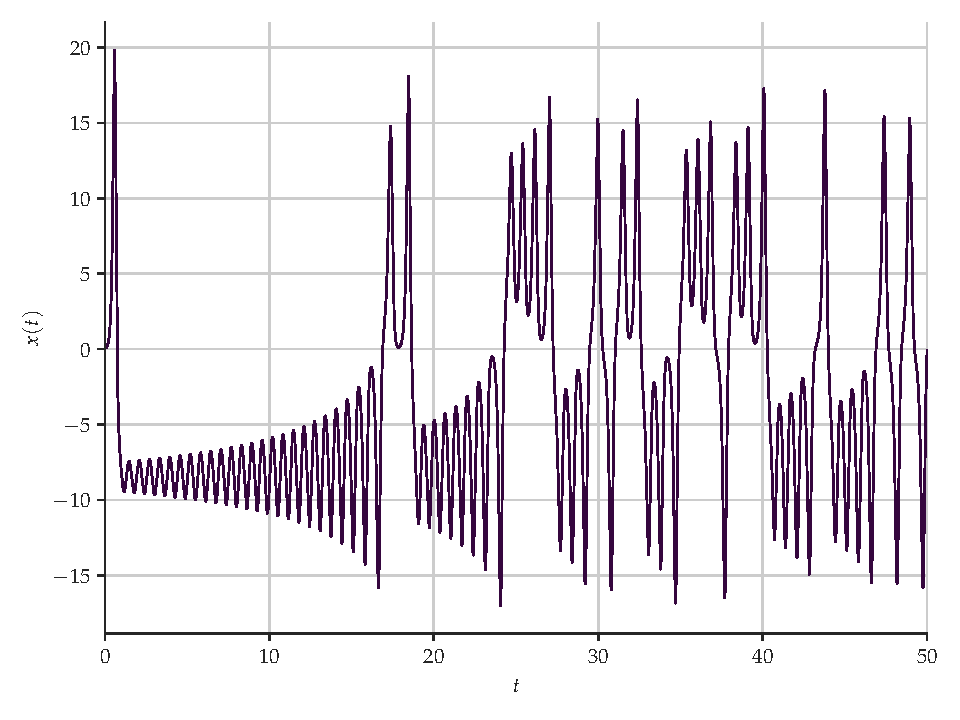
\includegraphics[scale=0.2]{serie-lorenz-x.pdf}
         %\caption{$y=5/x$}
     \end{subfigure}
     \centering
     \begin{subfigure}[t]{0.3\textwidth}
         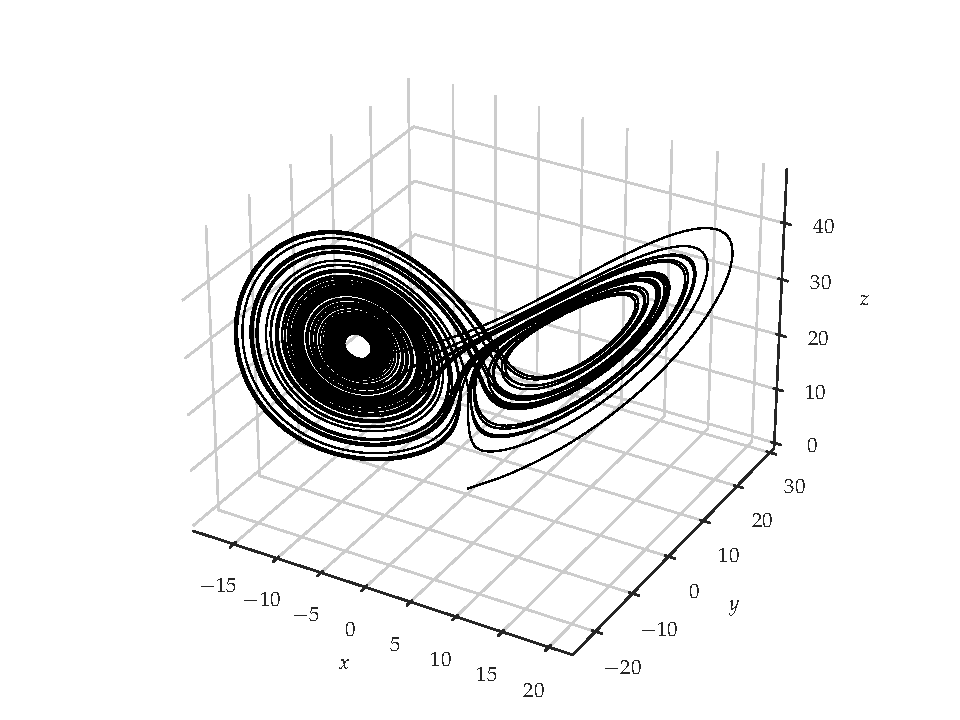
\includegraphics[scale=0.2]{diagrama-de-fases-lorenz.pdf}
         %\caption{$y=x$}
     \end{subfigure}
     \caption{À esquerda, a série temporal em $x$ do sistema de Lorenz simulado e, à direita, o diagrama de fases correspondente à simulação}
     \label{fig:lorenz}
\end{figure}
\end{frame}

\subsection{Equações de Mackey-Glass}
\begin{frame}
	\frametitle{Cenários escolhidos}
	\framesubtitle{Equações de Mackey-Glass}
	\justifying O último sistema caótico simulado está associado às equações de Mackey-Glass, as quais modelam o controle hormonal da produção de células brancas do sangue e podem ser vistas abaixo \cite{mackey1977oscillation}:
\begin{subequations}
\begin{equation}
\frac{dP(t)}{dt} = \frac{\beta_0\cdot \theta^n}{\theta^n + P(t - \tau)^n} - \gamma\cdot P(t)
\end{equation}
\begin{equation}\label{eq:mackey-glass-chaos}
\frac{dP(t)}{dt} = \frac{\beta_0\cdot \theta^n \cdot P(t - \tau)}{\theta^n + P(t - \tau)^n} - \gamma\cdot P(t)
\end{equation}
\end{subequations}
\end{frame}

\begin{frame}
	\frametitle{Cenários escolhidos}
	\framesubtitle{Equações de Mackey-Glass}
\justifying A equação (\ref{eq:mackey-glass-chaos}) exibe comportamento caótico para valores mais altos de $\tau$. Para a simulação numérica, foi utilizado $n = 10$, $\gamma = 0.1$, $\beta = 0.2$, $\theta = 1$, $\tau = 22$, $dt = 1.0$ e $P(0^-)=0.1$, gerando novamente $5000$ amostras. A série e o atrator obtidos podem ser vistos na figura \ref{fig:mackey-glass}.
\begin{figure}[H]
     \begin{subfigure}[t]{0.3\textwidth}
         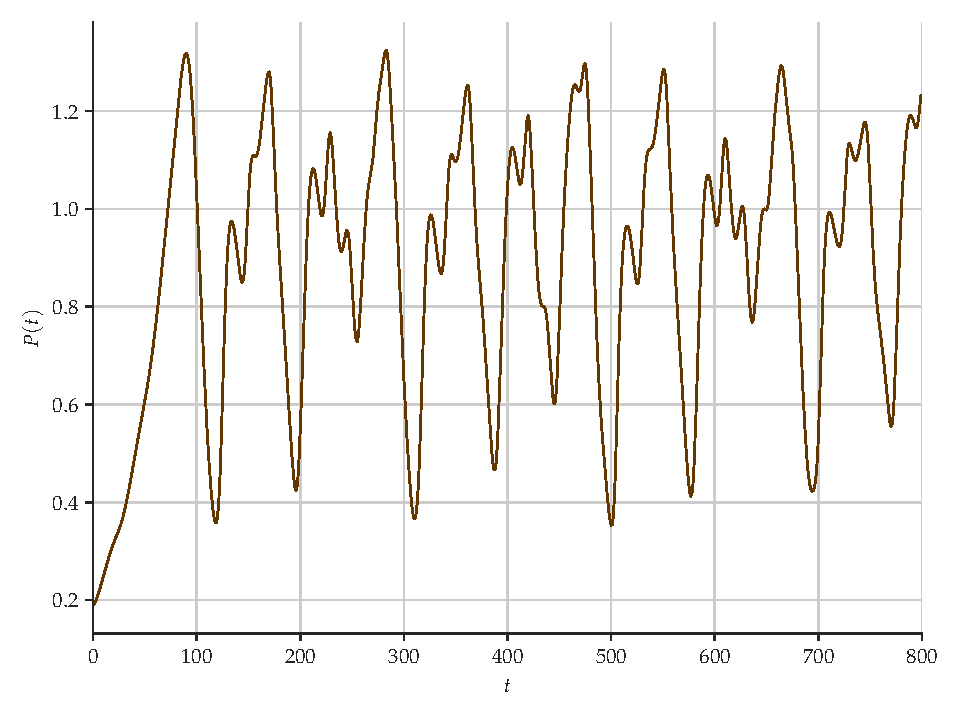
\includegraphics[scale=0.2]{serie-mackeyglass.pdf}
         %\caption{$y=5/x$}
     \end{subfigure}
     \centering
     \begin{subfigure}[t]{0.3\textwidth}
         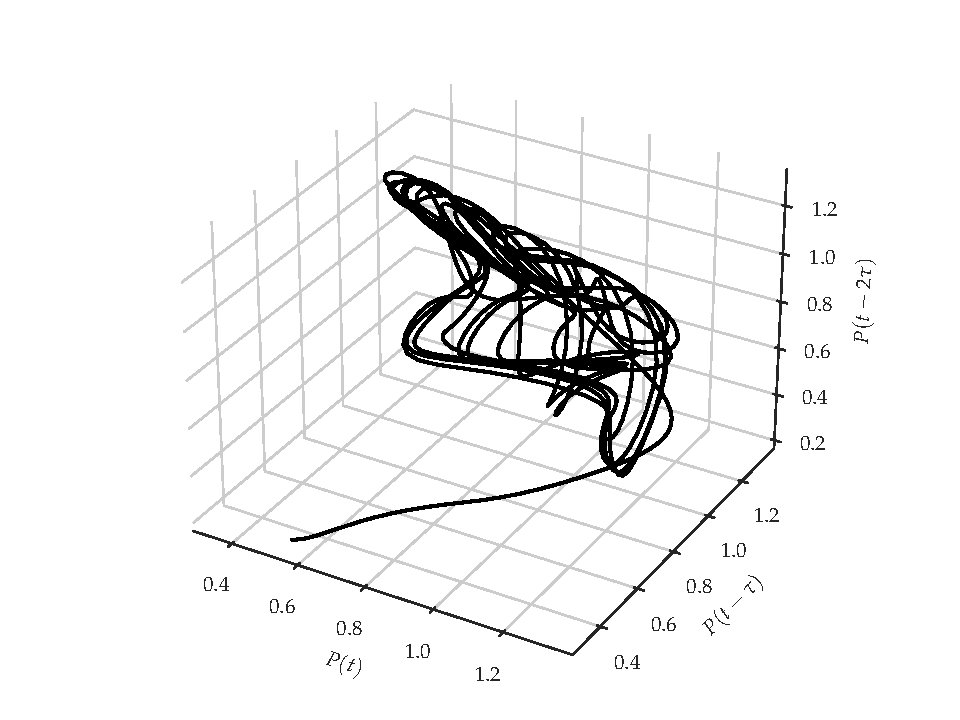
\includegraphics[scale=0.2]{atrator-mackeyglass.pdf}
         %\caption{$y=x$}
     \end{subfigure}
     \caption{À esquerda, a série temporal da equação (\ref{eq:mackey-glass-chaos}) exibida de $t = 0 $ a $t = 800$ e, à direita, o atrator correspondente à simulação}
     \label{fig:mackey-glass}
\end{figure}
\end{frame}

\section{Redes neurais utilizadas para a previsão}

\subsection{MLP}

\begin{frame}
\frametitle{Redes neurais utilizadas para a previsão}
\framesubtitle{MLP}
\justifying As redes MLP, como o nome já diz, são compostas por múltiplas camadas de neurônios artificiais do tipo \textit{perceptron}  \cite{rosenblatt1958perceptron}. Cada neurônio recebe os atributos $x_i, i = 1, \ldots, m$ de entrada e os pondera por pesos $w_i$. Em seguida, é aplicada uma função de ativação $\varphi(\cdot)$ sobre esta soma ponderada, acrescida de um termo de \textit{bias}, conforme indica a equação (\ref{eq:mlp-out}).
\begin{equation}\label{eq:mlp-out}
y = \varphi  \left(\sum_{i=1}^{m}w_i x_i + w_0 \right) = \varphi \left(\sum_{i=0}^{m}w_i x_i \right) = \varphi \left(\mathbf{w}^T \cdot \mathbf{x} \right)
\end{equation}
\end{frame}

\begin{frame}
\frametitle{Redes neurais utilizadas para a previsão}
\framesubtitle{MLP}
\justifying Uma rede neural MLP é composta por um número arbitrário $N_L$ de  camadas com $n$ neurônios do tipo \textit{perceptron}, com a característica de que as saídas dos neurônios da $l$-ésima camada são propagadas para a frente, servindo como as entradas de todos os neurônios da camada seguinte ($l+1$). A figura \ref{fig:mlp-architecture} apresenta a estrutura típica das redes MLP.
\begin{figure}[H]
\centering
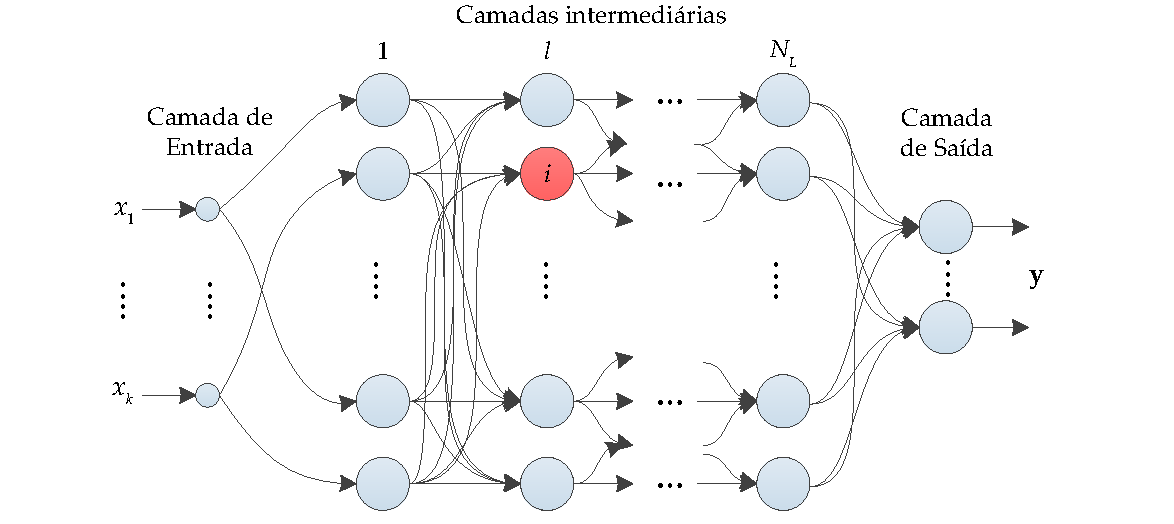
\includegraphics[scale = 0.3]{mlp-network.pdf}
\caption{Estrutura típica de uma rede MLP (figura adaptada de \cite{boccato2013novas}) }
\label{fig:mlp-architecture}
\end{figure}
\end{frame}

\begin{frame}
\frametitle{Redes neurais utilizadas para a previsão}
\framesubtitle{MLP}
\justifying O processo de treinamento de uma rede neural artificial normalmente é realizado com sequências de vetores de entrada $\mathbf{x}$, chamadas de \textit{mini-batch}, sendo que um período de treinamento é chamado de época \cite{geron2019hands}. 

Os pesos sinápticos $\textbf{w}$ são ajustados com um processo iterativo de forma a minimizar uma função custo $J(\textbf{w})$ que representa uma medida do erro entre as saídas geradas pela rede e as saídas desejadas. 
\end{frame}

\subsection{LSTM e GRU}

\begin{frame}
\frametitle{Redes neurais utilizadas para a previsão}
\framesubtitle{LSTM e GRU}
\justifying As redes recorrentes têm estruturas computacionais que podem armazenar os estados anteriores dos neurônios, possuindo também portas não-lineares que regulam o fluxo de informação de entrada e de saída da célula computacional \cite{haykin2010neural}. 

A diferença entre uma célula LSTM e uma célula GRU é a presença de um vetor de longo prazo $\mathbf{c}$ e um vetor de curto prazo $\mathbf{h}$ na LSTM, conforme indicado na figura \ref{fig:lstm-cell}. 

\centering
\begin{minipage}{0.3\textwidth}
\begin{figure}[H]
\begin{center}
\scalebox{0.3}{
\begin{tikzpicture}[
    % GLOBAL CFG
    font=\sf \scriptsize,
    >=LaTeX,
    % Styles
    cell/.style={% For the main box
        rectangle, 
        rounded corners=5mm, 
        draw,
        very thick,
        },
    operator/.style={%For operators like +  and  x
        circle,
        draw,
        inner sep=-0.5pt,
        minimum height =.2cm,
        },
    function/.style={%For functions
        ellipse,
        draw,
        inner sep=1pt
        },
    ct/.style={% For external inputs and outputs
        circle,
        draw,
        line width = .75pt,
        minimum width=1cm,
        inner sep=1pt,
        },
    gt/.style={% For internal inputs
        rectangle,
        draw,
        minimum width=4mm,
        minimum height=3mm,
        inner sep=1pt
        },
    mylabel/.style={% something new that I have learned
        font=\scriptsize\sffamily
        },
    ArrowC1/.style={% Arrows with rounded corners
        rounded corners=.25cm,
        thick,
        },
    ArrowC2/.style={% Arrows with big rounded corners
        rounded corners=.5cm,
        thick,
        }
    ]

%Start drawing the thing...    
    % Draw the cell: 
    \node [cell, minimum height =4cm, minimum width=6cm] at (0,0){} ;

    % Draw inputs named ibox#
    \node [gt] (ibox1) at (-2,-0.75) {$\sigma$};
    \node [gt] (ibox2) at (-1.5,-0.75) {$\sigma$};
    \node [gt, minimum width=1cm] (ibox3) at (-0.5,-0.75) {$\tanh$};
    \node [gt] (ibox4) at (0.5,-0.75) {$\sigma$};

   % Draw opérators   named mux# , add# and func#
    \node [operator] (mux1) at (-2,1.5) {$\times$};
    \node [operator] (add1) at (-0.5,1.5) {+};
    \node [operator] (mux2) at (-0.5,0) {$\times$};
    \node [operator] (mux3) at (1.5,0) {$\times$};
    \node [function] (func1) at (1.5,0.75) {$\tanh$};

    % Draw External inputs? named as basis c,h,x
    \node[] (c) at (-4,1.5) {$\mathbf{c}(t-1)$};
    \node[] (h) at (-4,-1.5) {$\mathbf{h}(t-1)$};
    \node[] (x) at (-2.5,-3) {$\mathbf{x}(t)$};

    % Draw External outputs? named as basis c2,h2,x2
    \node[] (c2) at (4,1.5) {$\mathbf{c}(t)$};
    \node[] (h2) at (4,-1.5) {$\mathbf{h}(t)$};
    \node[] (x2) at (2.5,3) {$\mathbf{y}(t)$};
    
    % Draw internals functions, named as basis fi,ii,ci,oi
    \node[] (fi) at (-2.35,-0.25) {$\mathbf{f}(t)$};
    \node[] (ii) at (-1.5,0.2) {$\mathbf{i}(t)$};
    \node[] (ci) at (-0.1,-0.35) {$\mathbf{\tilde{c}}(t)$};
	\node[] (oi) at (0.5,0.2) {$\mathbf{o}(t)$};       
    
% Start connecting all.
    %Intersections and displacements are used. 
    % Drawing arrows    
    \draw [ArrowC1] (c) -- (mux1) -- (add1) -- (c2);

    % Inputs
    \draw [ArrowC2] (h) -| (ibox4);
    \draw [ArrowC1] (h -| ibox1)++(-0.5,0) -| (ibox1); 
    \draw [ArrowC1] (h -| ibox2)++(-0.5,0) -| (ibox2);
    \draw [ArrowC1] (h -| ibox3)++(-0.5,0) -| (ibox3);
    \draw [ArrowC1] (x) -- (x |- h)-| (ibox3);

    % Internal
    \draw [->, ArrowC2] (ibox1) -- (mux1);
    \draw [->, ArrowC2] (ibox2) |- (mux2);
    \draw [->, ArrowC2] (ibox3) -- (mux2);
    \draw [->, ArrowC2] (ibox4) |- (mux3);
    \draw [->, ArrowC2] (mux2) -- (add1);
    \draw [->, ArrowC1] (add1 -| func1)++(-0.5,0) -| (func1);
    \draw [->, ArrowC2] (func1) -- (mux3);

    %Outputs
    \draw [->, ArrowC2] (mux3) |- (h2);
    \draw [->] (add1) |- (c2);
    \draw (c2 -| x2) ++(0,-0.1) coordinate (i1);
    \draw [-, ArrowC2] (h2 -| x2)++(-0.5,0) -| (i1);
    \draw [->, ArrowC2] (i1)++(0,0.2) -- (x2);

\end{tikzpicture}}
\end{center}
\caption{Estrutura de uma célula LSTM.}
\label{fig:lstm-cell}
\end{figure}
\end{minipage} \; \; \; \; \;
\begin{minipage}{0.3\textwidth}
\begin{figure}[H]
\begin{center}
\scalebox{0.3}{
\begin{tikzpicture}[
    % GLOBAL CFG
    font=\sf \scriptsize,
    >=LaTeX,
    % Styles
    cell/.style={% For the main box
        rectangle, 
        rounded corners=5mm, 
        draw,
        very thick,
        },
    operator/.style={%For operators like +  and  x
        circle,
        draw,
        inner sep=-0.5pt,
        minimum height =.2cm,
        },
    function/.style={%For functions
        ellipse,
        draw,
        inner sep=1pt
        },
    ct/.style={% For external inputs and outputs
        circle,
        draw,
        line width = .75pt,
        minimum width=1cm,
        inner sep=1pt,
        },
    gt/.style={% For internal inputs
        rectangle,
        draw,
        minimum width=4mm,
        minimum height=3mm,
        inner sep=1pt
        },
    mylabel/.style={% something new that I have learned
        font=\tiny\sffamily
        },
    ArrowC1/.style={% Arrows with rounded corners
        rounded corners=.25cm,
        thick,
        },
    ArrowC2/.style={% Arrows with big rounded corners
        rounded corners=.5cm,
        thick,
        }
    ]

%Start drawing the thing...    
    % Draw the cell: 
    \node [cell, minimum height =4cm, minimum width=6cm] at (0,0){} ;

    % Draw inputs named ibox#
    \node [gt] (ibox1) at (-1.5,-0.75) {$\sigma$};
    \node [gt] (ibox2) at (0,-1.2) {$\sigma$};

   % Draw opérators   named mux# , add# and func#
    \node [operator] (mux1) at (-1.5,0) {$\times$};
    \node [operator] (mux2) at (0,1.5) {$\times$};
    \node [operator] (mux4) at (2.5,0.75) {$\times$};
    \node [operator] (add1) at (2.5,1.5) {+};    
    \node [function] (func1) at (2.5,0) {$\tanh$};
    \node [operator] (min1) at (1.25,0.75) {{\scalebox{0.5}{$-1$}}};

    % Draw External inputs? named as basis c,h,x
    \node[] (h) at (-4,1.5) {$\mathbf{h}(n-1)$};
    \node[] (x) at (0,-3) {$\mathbf{x}(n)$};

    % Draw External outputs? named as basis c2,h2,x2
    \node[] (h2) at (4,1.5) {$\mathbf{h}(n)$};
    \node[] (x2) at (2.5,3) {$\mathbf{y}(n)$};
    
    % Draw internals functions, named as basis fi,ii,ci,oi
    \node[] (ri) at (-1.85,-0.35) {$\mathbf{r}(n)$};
    \node[] (zi) at (0.4,-0.85) {$\mathbf{z}(n)$};  
    \node[] (gi) at (2.1,0.4) {$\mathbf{g}(n)$}; 
    
% Start connecting all.
    %Intersections and displacements are used. 
    % Drawing arrows    
    \draw [->, ArrowC1] (h) -- (mux2);
    \draw [->, ArrowC1] (h -| ibox1)++(-1,0) |- (ibox1);

    % Inputs

    % Internal
    \draw [->, ArrowC2] (ibox1) -- (mux1);
    
    \draw [->, ArrowC2] (ibox2) -- (mux2);
    \draw [->, ArrowC2] (mux4) -- (add1);
    \draw [->, ArrowC2] (func1) -- (mux4);
   % \draw [->, ArrowC1] (add1 -| func1)++(-0.5,0) -| (func1);

    %Outputs
    \draw [ArrowC1, ->] (mux2) -- (add1);
    \draw [ArrowC1, ->] (add1) -- (h2);
    \draw (h2 -| x2) ++(0,-0.1) coordinate (i1);
    \draw [->, ArrowC1] (h -| mux1)++(-0.5,0) |- (mux1);
    %\draw (h -- mux1) ++(-2,2) coordinate (mux1);
    \draw [->, ArrowC2] (i1)++(0,0.2) -- (x2);
    \draw [->, ArrowC1] (x -| ibox1) ++ (+1.5,+1.25) -| (ibox1);
    \draw [->, ArrowC1] (x -| func1) ++ (-2.5,+1.25) -| (func1);
    \draw [->, ArrowC1] (x) -- (ibox2);
   % \draw [->, ArrowC1] (mux1) -- (func1);
    \draw [->, ArrowC2] (mux1 -| func1)++(-2.4,0) -- (func1) coordinate (i1);
    \draw [ArrowC1] (mux1) -- ++(+1.4,0);
    \draw [->, ArrowC1] (min1) -- (mux4);
    \draw [->, ArrowC1] (ibox2) |- (min1);

\end{tikzpicture}}
\end{center}
\caption{Estrutura de uma célula GRU.}
\label{fig:gru-cell}
\end{figure}
\end{minipage}
\end{frame}

\begin{frame}
\frametitle{Redes neurais utilizadas para a previsão}
\framesubtitle{LSTM e GRU}
\justifying À semelhança das redes MLP, o treinamento das redes LSTM e GRU também é realizado através de algoritmos de otimização baseados em derivadas da função custo; a diferença é que agora é necessário propagar as derivadas ao longo da estrutura e, também, ao longo do tempo devido às realimentações \cite{geron2019hands}. 
\end{frame}

\subsection{ESN}

\begin{frame}
\frametitle{Redes neurais utilizadas para a previsão}
\framesubtitle{ESN}
\justifying As redes neurais com estados de eco também são modelos recorrentes para processamento da informação, à semelhança da LSTM e da GRU. No entanto, apresentam um modo de operação e um esquema de treinamento bem diferentes  \cite{boccato2013novas}. 

A figura \ref{fig:esn-model} apresenta a estrutura interna de uma rede ESN.
\begin{figure}[H]
\centering
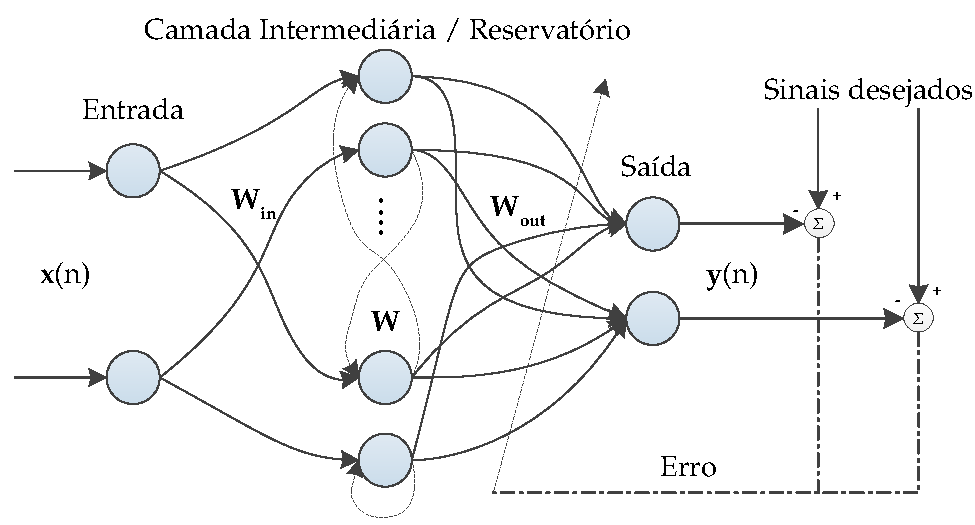
\includegraphics[scale = 0.35]{esn-network.pdf}
\caption{Estrutura típica de uma rede ESN (figura adaptada de \cite{boccato2013novas}).}
\label{fig:esn-model}
\end{figure}
\end{frame}

\begin{frame}
\frametitle{Redes neurais utilizadas para a previsão}
\framesubtitle{ESN}
\justifying O grande diferencial prático desta rede é que os pesos das conexões recorrentes dentro do reservatório $\mathbf{W}$ são ajustados com valores fixos antes do treinamento da camada de saída. Esses parâmetros são determinados tendo em vista a propriedade de estados de eco, existindo alguns métodos simples para a criação aleatória dos pesos e que asseguram a propriedade, conforme demonstrado em \cite{jaeger2007echo}. 
\end{frame}

\section{Metodologia}

\begin{frame}
\frametitle{Metodologia}
\justifying Iniciamos a análise através de um processo de busca em grade para determinarmos os parâmetros ótimos das redes neurais em cada cenário. 

Em seguida, avaliamos a progressão do erro quadrático médio (EQM) em função do número de amostras de entrada do modelo preditor (chamado de $K$). 
\end{frame}

\begin{frame}
\frametitle{Metodologia}
\justifying Por fim, comparamos qual foi a média e o desvio padrão do EQM com o melhor valor de $K$ de cada modelo nos quatro cenários. O horizonte de predição utilizado foi $L=3$. Assim, iremos predizer o valor da terceira iteração à frente do valor atual da série temporal.
\end{frame}

\subsection{Configurações das redes neurais}

\begin{frame}
\frametitle{Metodologia}
\framesubtitle{Configurações das redes neurais}
\justifying Para cada arquitetura, um conjunto de valores candidatos foi gerado para cada hiperparâmetro e todas as combinações possíveis foram avaliadas tendo em vista o desempenho do modelo em dados de validação, utilizando um processo de busca em grade.

Mais detalhes podem ser vistos no artigo enviado ao congresso.
\end{frame}

\subsection{Análise do melhor valor para $K$}

\begin{frame}
\frametitle{Metodologia}
\framesubtitle{Análise do melhor valor para $K$}
\justifying 

Com as melhores configurações para cada rede e cenário obtidas, foi analisada a progressão do erro quadrático médio para cada valor de $K$. A faixa de valores para $K$ a ser testada foi determinada utilizando a autocorrelação parcial das séries temporais de cada sistema analisado, levando em consideração os valores de $K$ que têm as autocorrelações parciais mais relevantes.
\end{frame}

\begin{frame}
\frametitle{Metodologia}
\framesubtitle{Análise do melhor valor para $K$}
\justifying 
Para realizar esse procedimento, cada rede (com as configurações ótimas) foi treinada utilizando $85\%$ dos dados gerados, sendo que $10\%$ dos dados de treinamento foi utilizado como o conjunto de validação (nas redes MLP, LSTM e GRU). Em seguida, foi avaliado o EQM no conjunto de teste (que corresponde às últimas 750 amostras). Esse processo foi realizado $5$ vezes para cada $K$, obtendo assim um valor médio e desvio-padrão para cada modelo e em cada cenário. 
\end{frame}

\begin{frame}
\frametitle{Metodologia}
\framesubtitle{Análise do melhor valor para $K$}
\justifying 
A figura \ref{fig:mse-progression} mostra a progressão do EQM observada em cada cenário. 
\begin{figure}[H]
     \begin{subfigure}[t]{0.4\textwidth} 
     \centering
         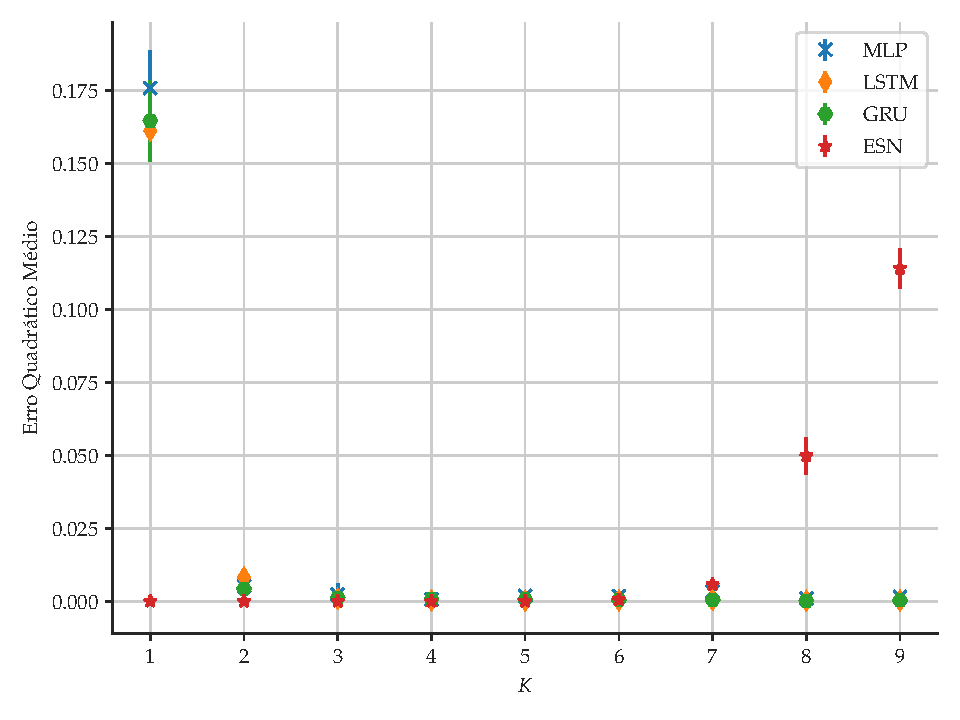
\includegraphics[scale=0.17]{progressao-k-henon.pdf}
         \caption{Mapa de Hénon}
     \end{subfigure}
     \centering
     \begin{subfigure}[t]{0.4\textwidth} 
     \centering
         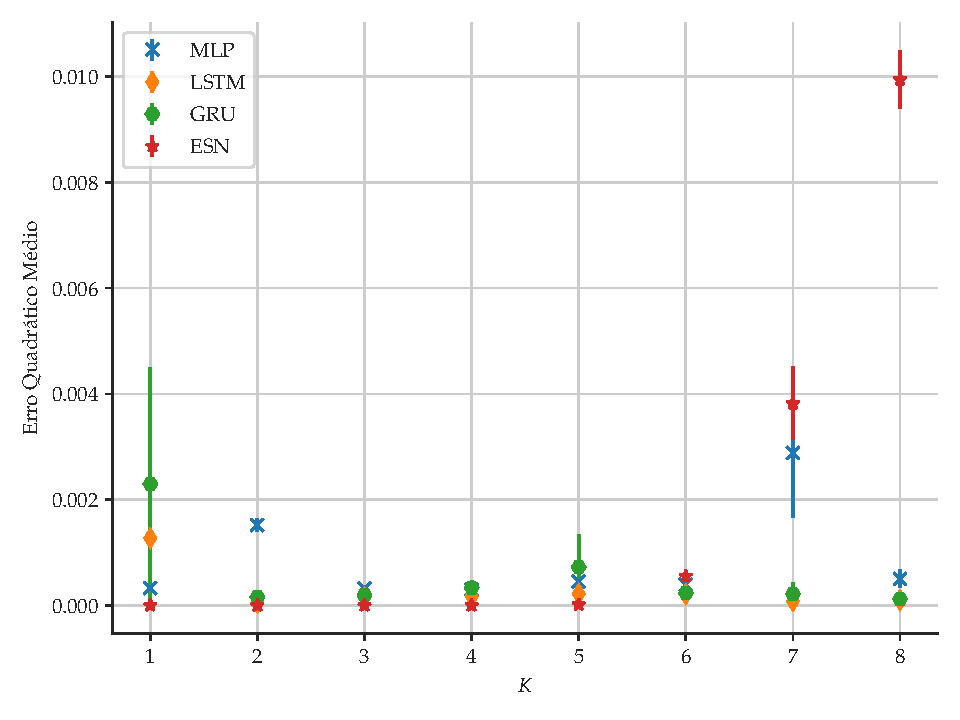
\includegraphics[scale=0.17]{progressao-k-logistic.pdf}
         \caption{Mapa logístico}
     \end{subfigure}
     \centering
     \\
     \begin{subfigure}[t]{0.4\textwidth}
     \centering
         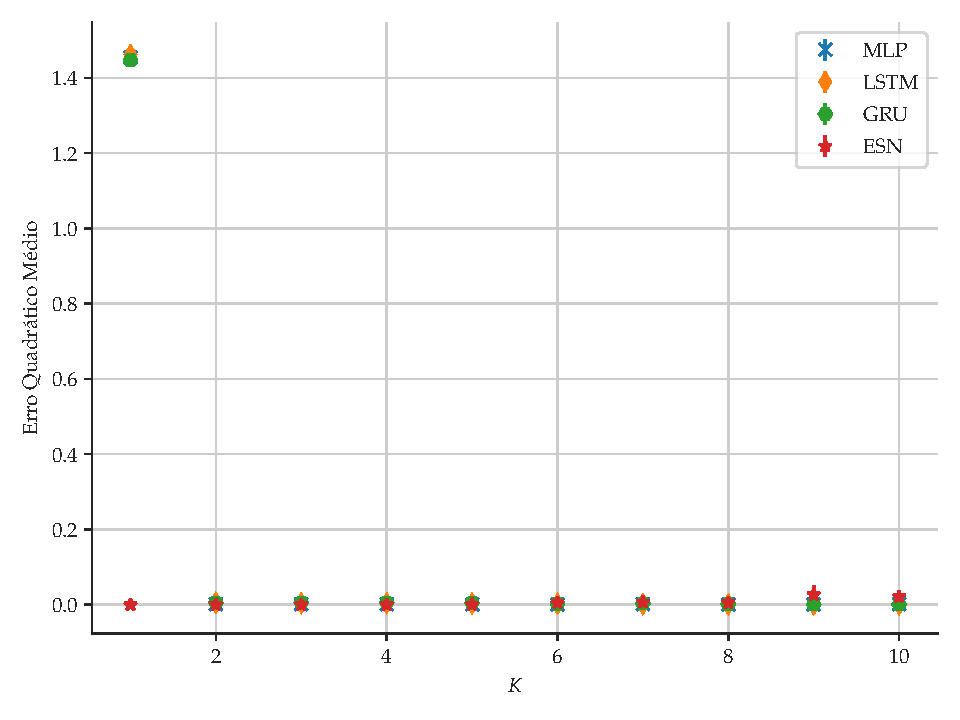
\includegraphics[scale=0.17]{progressao-k-lorenz.pdf}
         \caption{Sistema de Lorenz}
     \end{subfigure}
     \centering
     \begin{subfigure}[t]{0.4\textwidth} 
     \centering
         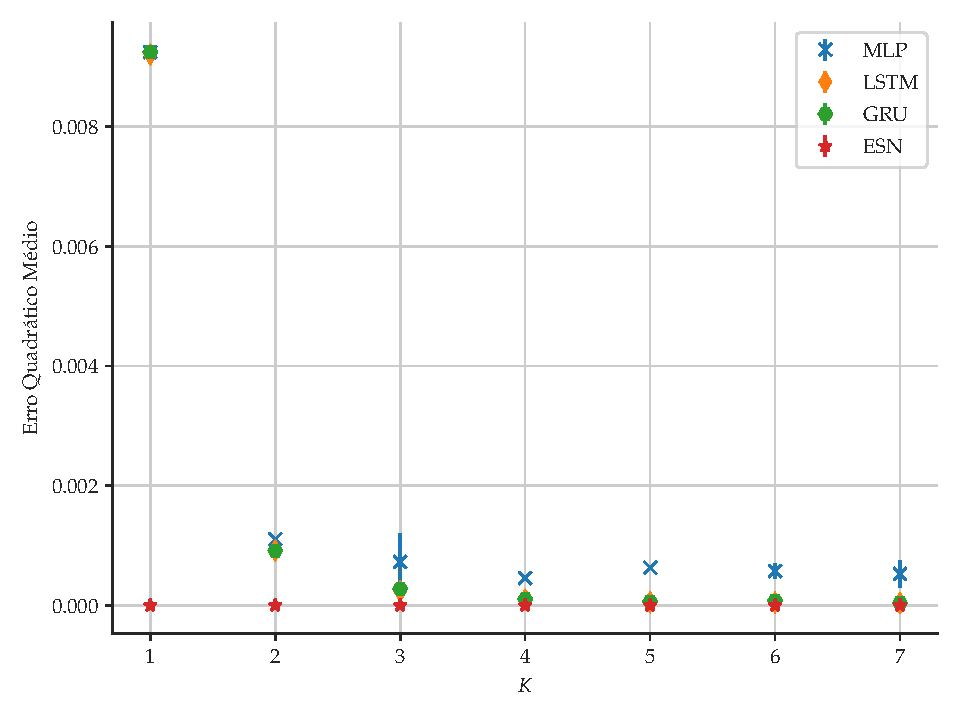
\includegraphics[scale=0.17]{progressao-k-mackeyglass.pdf}
         \caption{Equações de Mackey-Glass}
     \end{subfigure}  
     \centering   
     \caption{Progressão do erro quadrático médio para cada valor de $K$.}
     \label{fig:mse-progression}
\end{figure}
\end{frame}

\section{Resultados}

\begin{frame}
\frametitle{Resultados}
\justifying Após identificarmos o melhor valor de $K$ para cada modelo, realizou-se novamente o processo mencionado na seção anterior e foi obtido o EQM para as melhores configurações (parâmetros e $K$) para cada modelo, em todos os cenários. 
\end{frame}

\begin{frame}
\frametitle{Resultados}
\justifying A figura \ref{fig:model-comparison} exibe o comparativo dos desempenhos obtidos por cada modelo com as melhores configurações nos cenários testados.
\begin{figure}[!h]
     \begin{subfigure}[t]{0.4\textwidth}
     	\centering
         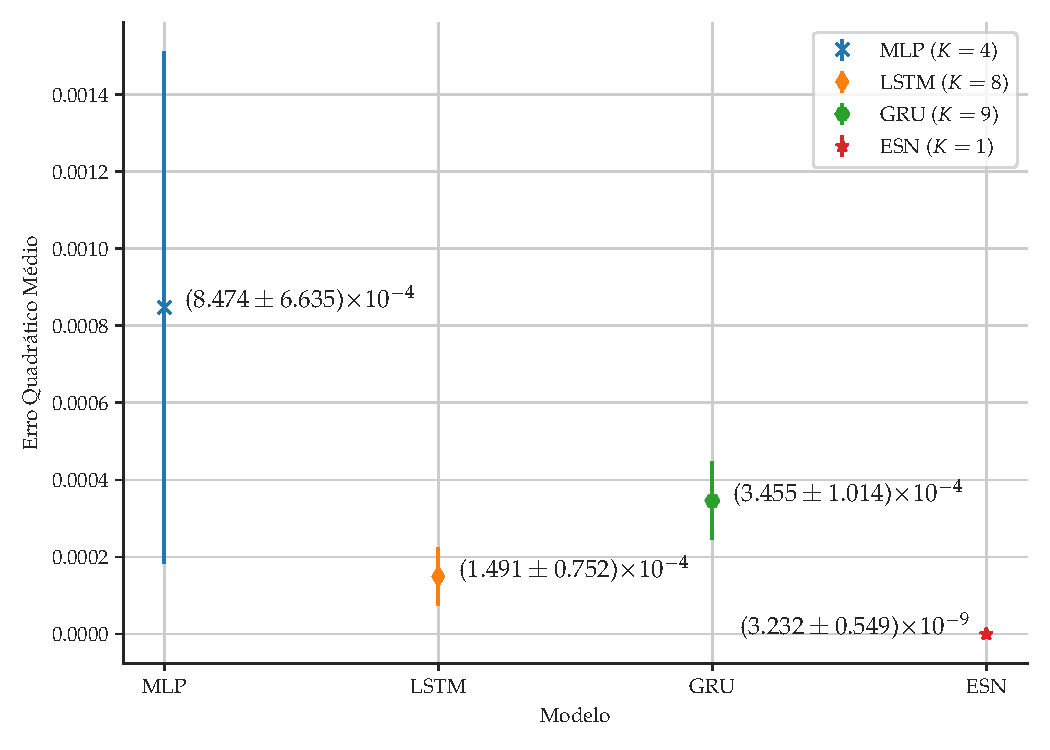
\includegraphics[scale=0.15]{comparacao-k-henon.pdf}
         \caption{Mapa de Hénon}
     \end{subfigure}
     \centering
     \begin{subfigure}[t]{0.4\textwidth} 
     \centering
         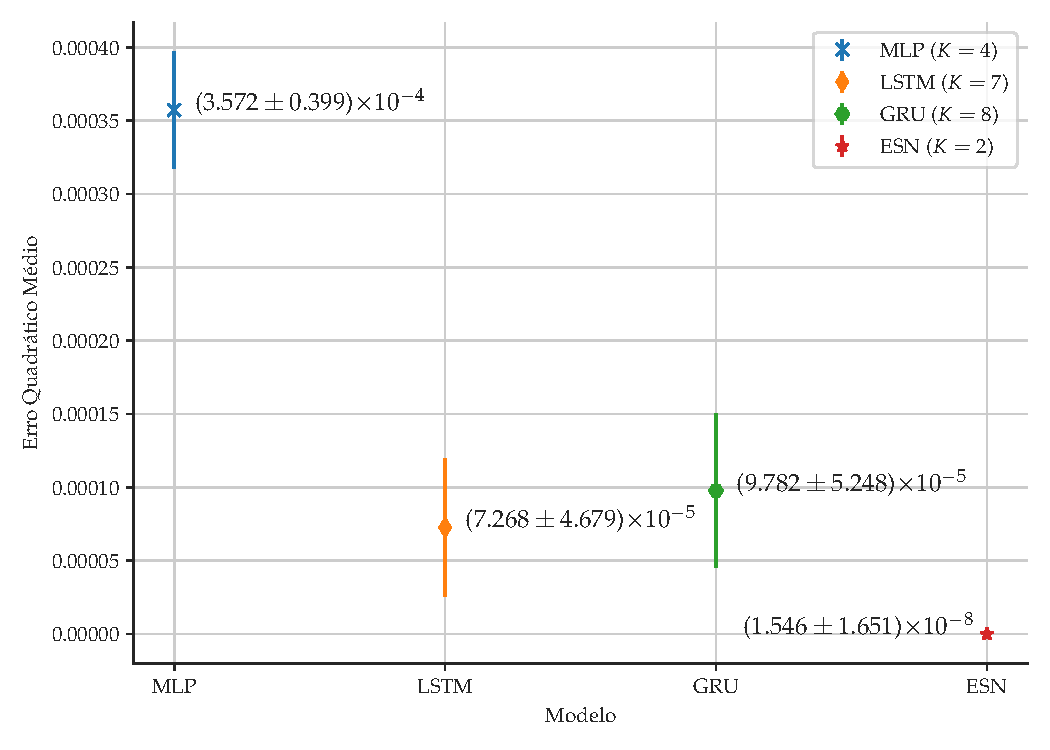
\includegraphics[scale=0.15]{comparacao-k-logistic.pdf}
         \caption{Mapa logístico}
     \end{subfigure}
     \centering\\
     \begin{subfigure}[t]{0.4\textwidth}
     \centering
         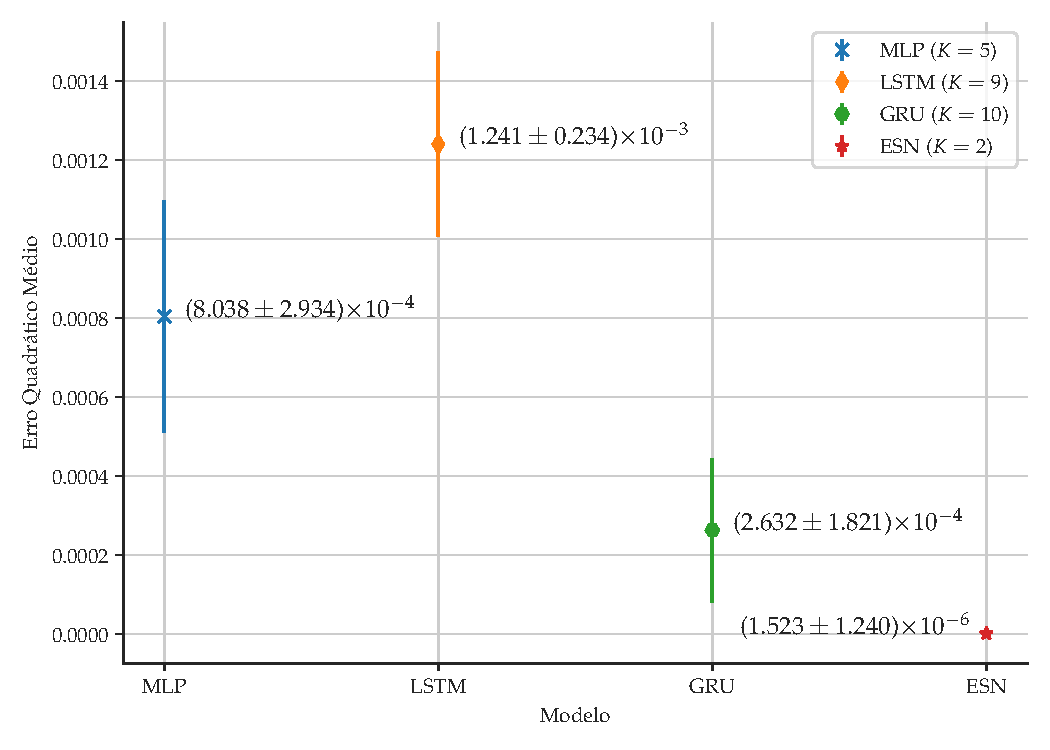
\includegraphics[scale=0.15]{comparacao-k-lorenz.pdf}
         \caption{Sistema de Lorenz}
     \end{subfigure}
     \centering
     \begin{subfigure}[t]{0.4\textwidth} 
     \centering
         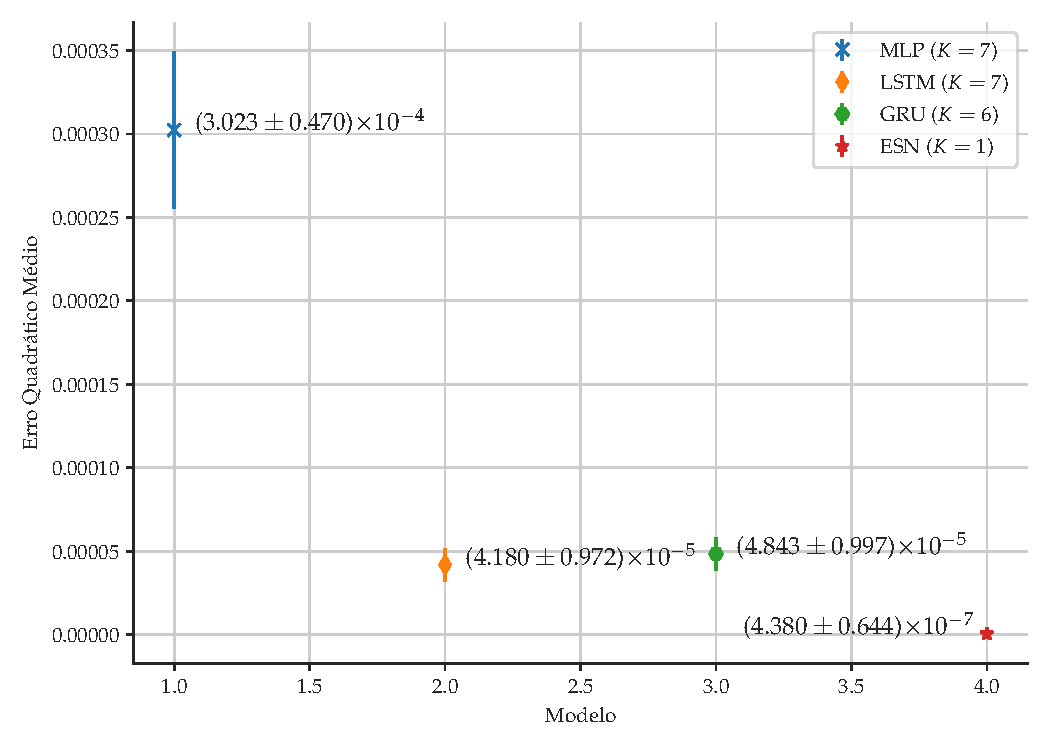
\includegraphics[scale=0.15]{comparacao-k-mackeyglass.pdf}
         \caption{Equações de Mackey-Glass}
     \end{subfigure}  
     \centering   
     \caption{Comparação do desempenho obtido por cada modelo.}
     \label{fig:model-comparison}
\end{figure}
\end{frame}

\begin{frame}
\frametitle{Resultados}
\justifying A figura \ref{fig:series-comparison} mostra uma comparação da predição em si de cada modelo nos cenários onde a diferença foi mais perceptível visualmente.

\begin{figure}[!ht]
     \begin{subfigure}[t]{0.4\textwidth} 
     \centering
         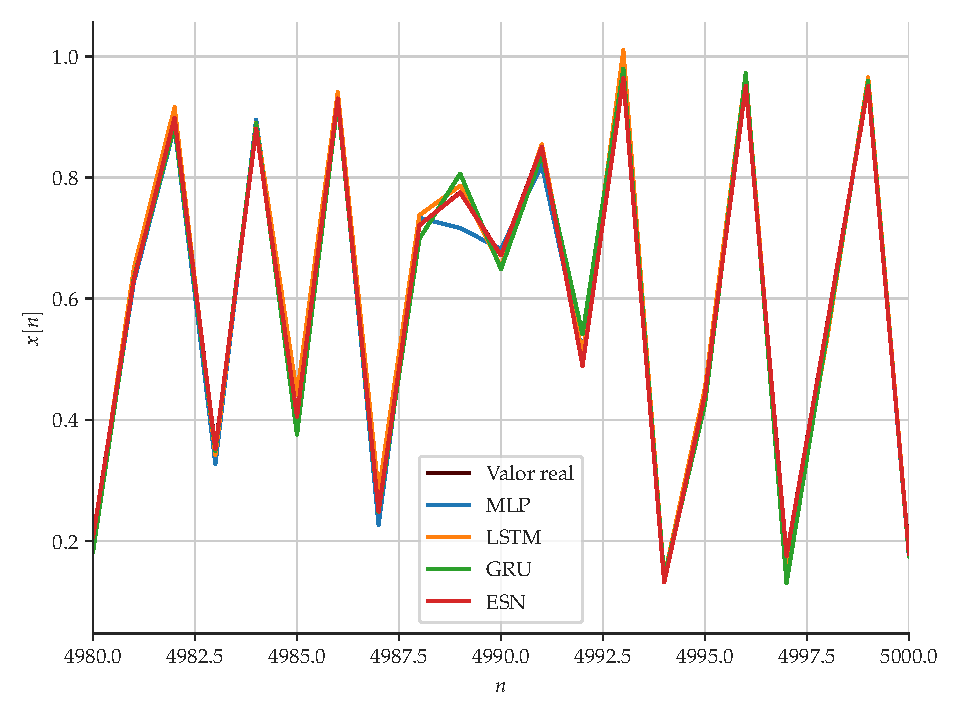
\includegraphics[scale=0.24]{vs-logistic-zoom.pdf}
         \caption{Mapa logístico}
     \end{subfigure}
     \centering
     \begin{subfigure}[t]{0.4\textwidth}
     \centering
         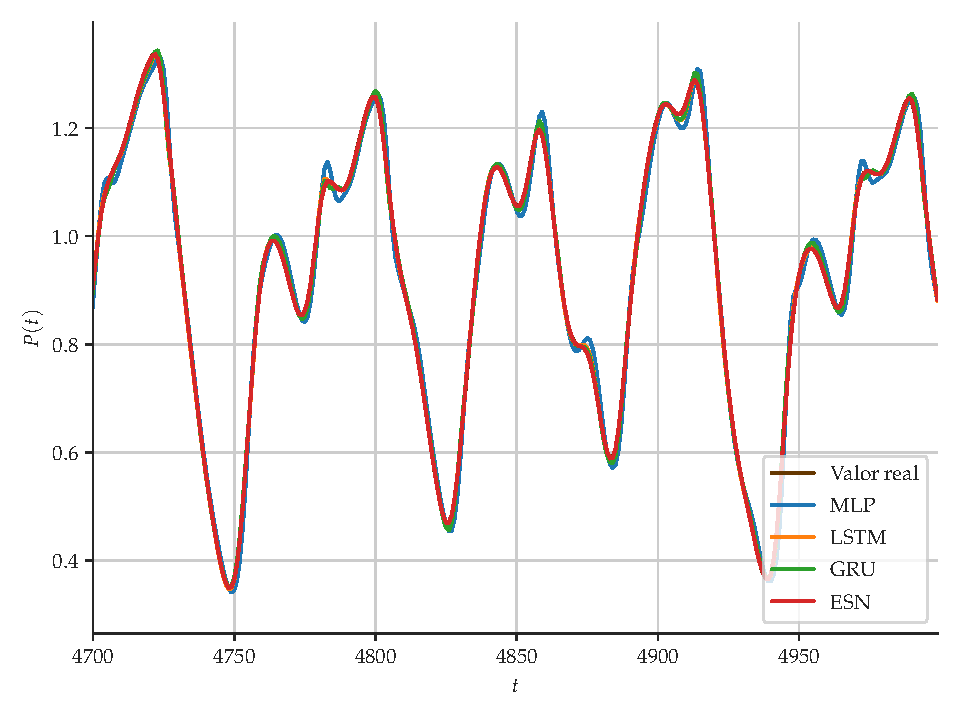
\includegraphics[scale=0.24]{vs-mackeyglass-zoom.pdf}
         \caption{Equações de Mackey-Glass}
     \end{subfigure}
     \centering     
     \caption{Comparação da predição realizada por cada modelo nos cenários do mapa logístico e das equações de Mackey-Glass.}
     \label{fig:series-comparison}
\end{figure}
\end{frame}

\section{Análise e Conclusão}

\begin{frame}
\frametitle{Análise e Conclusão}

\justifying Analisando os resultados obtidos, tiramos algumas conclusões importantes:

    \begin{itemize}[<+-| alert@+>]   
    \item A rede MLP foi consideravelmente pior do que as redes recorrentes,
    \item Dentre as redes recorrentes, a ESN obteve um EQM bem inferior ao obtido pela LSTM e pela GRU, 
    \item A ESN  atingiu patamares de erro cerca de $100$ ou até $10000$ vezes menores que os outros modelos.
    \end{itemize}
\end{frame}

\begin{frame}
\frametitle{Análise e Conclusão}
\justifying O desempenho inferior da rede MLP com relação às redes recorrentes provavelmente decorre do fato de que a relação temporal presente na LSTM, GRU e ESN auxilia na modelagem da dinâmica da série temporal. Já o pior desempenho da LSTM na série temporal do sistema de Lorenz provavelmente está relacionado aos efeitos estocásticos presentes no ajuste dos pesos sinápticos dessa rede neural que, conforme indicado em \cite{doya1992bifurcations}, é uma dificuldade em seu treinamento.
\end{frame}

\begin{frame}
\frametitle{Análise e Conclusão}
\justifying Considerando que a ESN obteve, de longe, o melhor desempenho, e que o treinamento desta arquitetura é bem menos custoso computacionalmente se comparado às demais, pode-se concluir que esta rede é uma boa alternativa para futuros estudos de modelos preditores de séries temporais. 
\end{frame}

\begin{frame}
\frametitle{Análise e Conclusão}
\justifying Além disso, conforme mostrado em outros trabalhos como \cite{jaeger2004harnessing, jaeger2007echo, boccato2013novas}, a ESN também é uma boa ferramenta para outras tarefas de extração de informação, como em equalização de canais e separação de fontes. 
\end{frame}

\begin{frame}
\frametitle{Análise e Conclusão}
\justifying Como sugestão de trabalhos futuros, pode ser avaliada a eficácia da ESN em reconstruir atratores através de séries temporais experimentais de sistemas caóticos. Se o desempenho para essa tarefa for tão bom quanto o obtido na predição das séries estudadas, a ESN pode tornar-se uma ferramenta ainda mais poderosa para a modelagem de sistemas com dinâmica caótica.
\end{frame}

\appendix

\begin{frame}[allowframebreaks]{Referências}
    \tiny
    \bibliography{bib}
    \bibliographystyle{ieeetr}
\end{frame}

\begin{frame}[plain,c]
    \begin{center}
    \Huge Muito Obrigado!
    \end{center}
\end{frame}


\end{document}
